
\section{削除された原子を色分け表示}
岩佐の研究で取り入れた原子の削除操作で,削除された原子の位置を視覚的に把握しやすくするためにおこなった.
図は削除の有無で色分けされた原子配置の三面図である.

\begin{figure}[htbp]\begin{center}
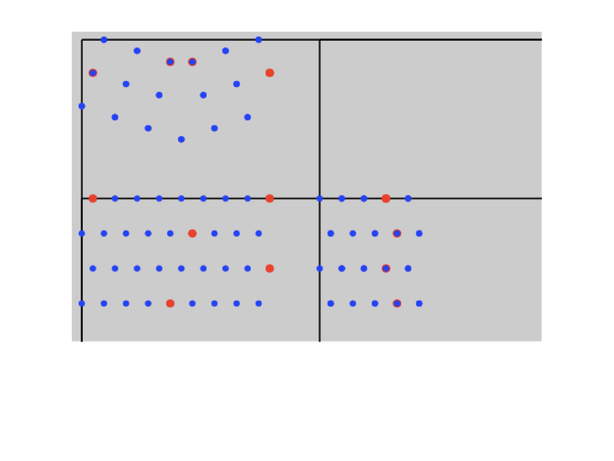
\includegraphics[width=6cm,bb=0 0 442 500]{../figs/./boundary_narita.010.jpg}
\caption{}
\label{default}\end{center}\end{figure}
赤い球が削除された原子に相当する.
viewerで表示することにより,削除された原子の数,並びに各々の配置をすぐに把握することが可能である.

\section{構造緩和による原子移動の表示}
再安定の原子配列にするために構造緩和をおこなう.
構造緩和によって移動した原子の位置を三面図で表示した.

\begin{figure}[htbp]\begin{center}
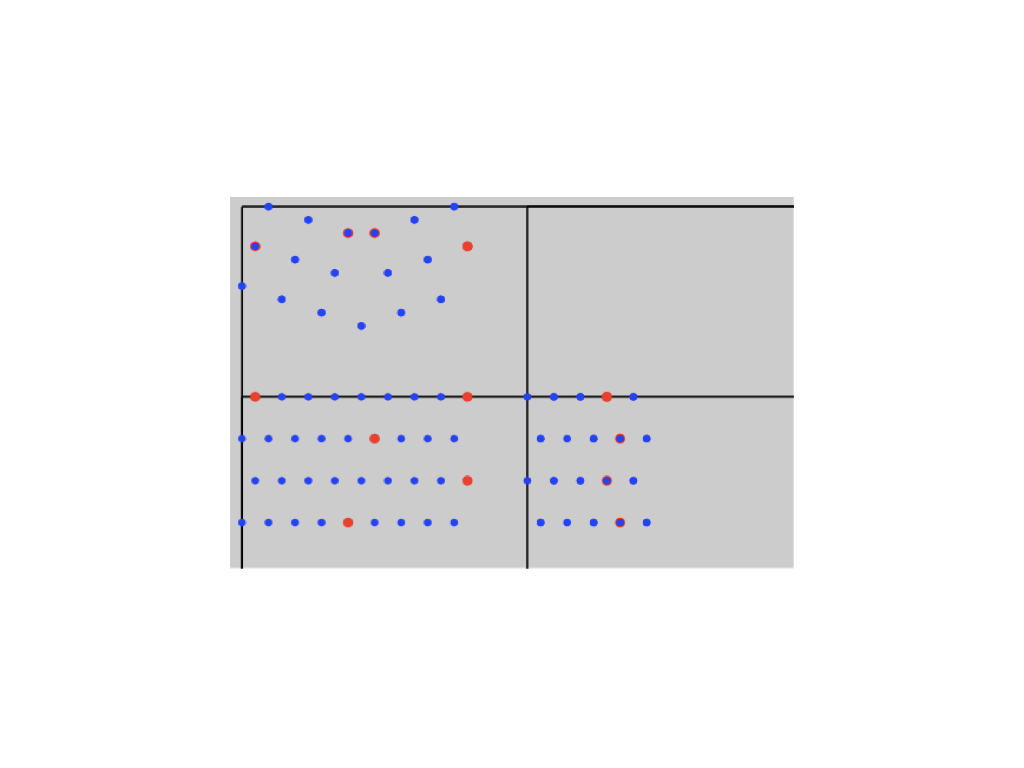
\includegraphics[width=6cm,bb=0 0 442 500]{../figs/./boundary_narita.011.jpg}
\caption{}
\label{default}\end{center}\end{figure}
図中の緑線は,構造緩和する前後で粒界原子が移動した軌道である.

\section{指定した層の白抜き表示}
POSCAR\_2223は4層の原子配列で構成されているため,原子配列を上から見た図,すなわち平面図では,原子同士が重なって配置してしまう.
したがって,指定した層の原子が上から見てどこに位置するのかを視覚的に確認できるために原子の白抜き処理をおこなった.

\begin{figure}[htbp]\begin{center}
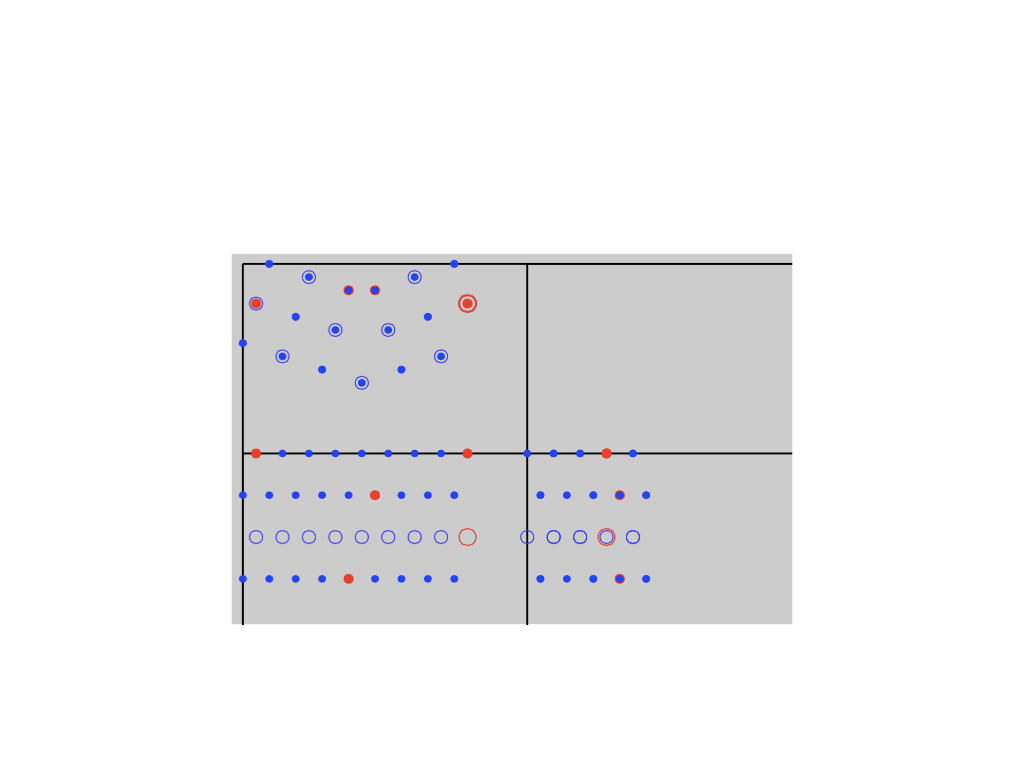
\includegraphics[width=6cm,bb=0 0 442 500]{../figs/./boundary_narita.012.jpg}
\caption{}
\label{default}\end{center}\end{figure}
図は,三層目を白抜きしたものである.

\section{三面図表示による改善点}
viewerによって三方向の視点で原子配列を表示した結果,構造緩和をおこなうためのPOSCARファイルに原子が一つ不足していることが分かった.
不足していた原子位置は,図13の赤枠部分である.

\begin{figure}[htbp]\begin{center}
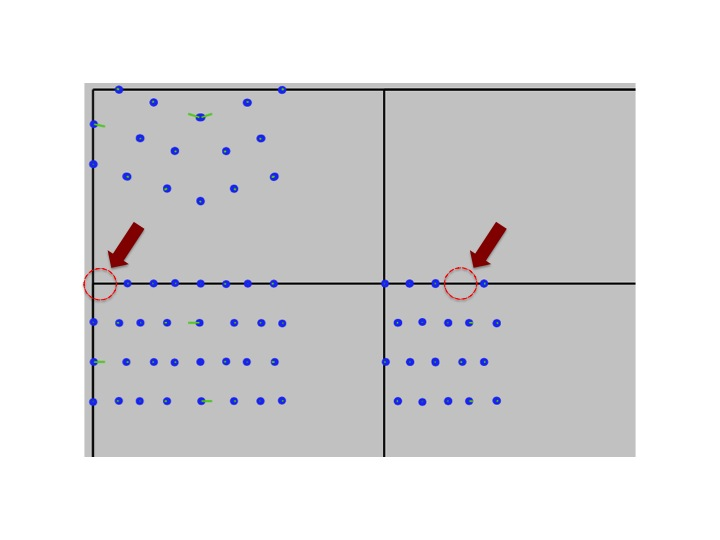
\includegraphics[width=6cm,bb=0 0 442 500]{../figs/./boundary_narita.013.jpg}
\caption{}
\label{default}\end{center}\end{figure}
これまでは,結晶構造描画ソフト"VESTA"を使用していたため,原子の細かい位置が確認できず,原子が不足していることを発見できなかった.
この結果により,構造緩和をおこなうためのPOSCARファイルに過ちがあったことを発見することができた.

\section{今後の課題}
本研究の結果を得て,

